	\chapter{Introduction to Deep Neural Networks}
	\section{Frequently Asked Questions}
	\resetquestioncounter{}
	\begin{qanda}
		\begin{question}
What is a Neural Network?
		\end{question}
		\begin{answer}
Neural Networks replicate the way humans learn, inspired by how the neurons in our brains fire, only much simpler.

The most common Neural Networks consist of three network layers:
	\begin{bulletedlist}
		\item An input layer
		\item A hidden layer (this is the most important layer where feature extraction takes place, and adjustments are made to train faster and function better).
		\item An output layer
	\end{bulletedlist}
 Each sheet contains neurons called ``nodes,'' performing various operations. Neural Networks are used in deep learning algorithms like CNN, RNN, GAN, etc.
		\end{answer}
	\end{qanda}


	\begin{qanda}
		\begin{question}
			What are hyperparameters?
		\end{question}
		\begin{answer}
With neural networks, you're usually working with hyperparameters once the data is formatted correctly. A hyperparameter is a parameter whose value is set before the learning process begins. It determines how a network is trained and the structure of the network (such as the number of hidden units, the learning rate, epochs, etc.).
		\end{answer}
	\end{qanda}


	\begin{qanda}
		\begin{question}
How to install TensorFlow 2.0 on Windows?
		\end{question}
		\begin{answer}
Open the Anaconda prompt and run the following code
\textcode{pip install tensorflow==2.8.0 --user}

Open the jupyter notebook, and refresh the page. Now, check the version of the TensorFlow by importing it with the following code in the jupyter notebook.

\textcode{import tensorflow as tf}
\textcode{print(tf.\_\_version\_\_)}
		\end{answer}
	\end{qanda}


	\begin{qanda}
		\begin{question}
How to install TensorFlow 2.0 on Mac?
		\end{question}
		\begin{answer}
Open your jupyter notebook in your Mac
To install TensorFlow, use the below command and run
\textcode{pip install tensorflow==2.8.0}

Open the jupyter notebook, and refresh the page. Now, check the version of the TensorFlow by importing it with the following code in the jupyter notebook.
\textcode{import tensorflow as tf}
\textcode{print(tf.\_\_version\_\_)}
		\end{answer}
	\end{qanda}


	\begin{qanda}
		\begin{question}
How to resolve the following error while importing Tensorflow?
		\end{question}
		\begin{answer}
``ImportError: DLL load failed: The specified module could not be found''

You can solve this error by downloading and installing visual studio 2015-2019 x86 and x64 from here (Links to an external site.)

Another solution is downgrading the TensorFlow version to 2.0:

\textcode{pip install tensorflow==2.0}

		\end{answer}
	\end{qanda}


	\begin{qanda}
		\begin{question}
What are activation functions?
		\end{question}
		\begin{answer}
In simple terms, an artificial neuron calculates the `weighted sum' of its inputs and adds a bias.

Now the value of net input can be anything from -8 to +8. The neuron doesn't really know how to bound to value and thus is not able to decide the firing pattern. Thus the activation function is an important part of an artificial neural network. They basically decide whether a neuron should be activated or not. Thus it bounds the value of the net input.  The activation function is a non-linear transformation that we do over the input before sending it to the next layer of neurons or finalizing it as output.
		\end{answer}
	\end{qanda}


	\begin{qanda}
		\begin{question}
What are the Softmax and ReLU Functions?
		\end{question}
		\begin{answer}
Softmax is an activation function that generates the output between zero and one. It divides each output, such that the total sum of the outputs is equal to one. Softmax is often used for output layers.

ReLU (or Rectified Linear Unit) is the most widely used activation function. It gives an output of X if X is positive and zeroes otherwise. ReLU is often used for hidden layers.%
		\end{answer}
	\end{qanda}

	\begin{qanda}
		\begin{question}
What is the meaning of back propagation?
		\end{question}
		\begin{answer}
Back propagation is a technique to improve the performance of the network. It back-propagates the error and updates the weights to reduce the error.
		\end{answer}
	\end{qanda}

	\begin{qanda}
		\begin{question}
What is Gradient Descent?
		\end{question}
		\begin{answer}
Gradient Descent is an optimal algorithm to minimize the cost function or to minimize an error. The aim is to find the local-global minima of a function. This determines the direction the model should take to reduce the error.
		\end{answer}
	\end{qanda}

	\section{Machine Learning versus Deep Learning}

	\begin{bulletedlist}
		\item Deep Learning is an important part of Machine Learning concerned with various algorithms which are inspired by the structure and function of brain called artificial
neural networks.
		\item Deep Learning is considered over traditional machine learning in many instances. The main reason for this is that the deep learning algorithms tries to learn and process very
high level of features from data and importantly unstructured data. So this is one of the greatest feature of deep learning over machine learning thus reducing the task of developing new feature extractors for every problem.
	\end{bulletedlist}

	\begin{topcaptiontable}
        \centering
        \lecaption{}
        \label{tab:}
		\begin{tabular}{|p{0.5\qandatextwidth-2\tabcolsep}|p{0.5\qandatextwidth-2\tabcolsep}|} \hline
				\tablecolumnheadervlinesone{Machine Learning} & \tablecolumnheadervlinestwo{Deep Learning} \\ \hline
				It can easily train on lesser data and requires lesser time to train. &
				It requires large data and longer time to train. \\ \hline
				It trains on CPU. &
				It trains on GPU. \\ \hline
				Some ML algorithms can be easily interpreted. &
				Difficult to interpret. \\ \hline%
		\end{tabular}
	\end{topcaptiontable}

	\begin{figure}[h]
		\centering
		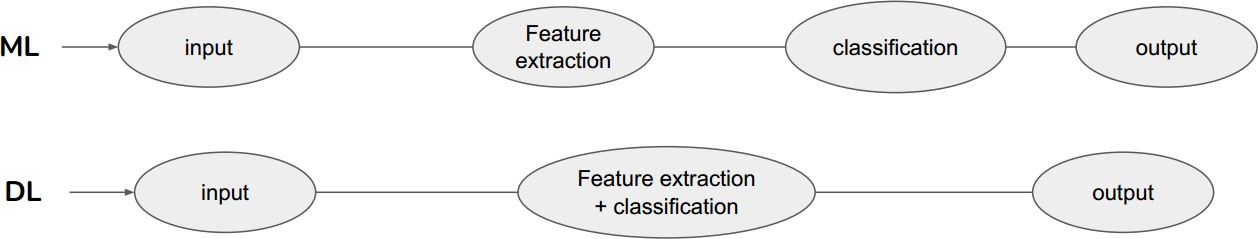
\includegraphics[width=0.85\textwidth]{machineversusdeeplearning}
		\caption{.}
		\label{fig:machineversusdeeplearning}
	\end{figure}


	\section{Using File with Google Colab}

	\begin{numberedlist}
		\item Open your drive, create a folder, and upload the data set and notebook in the folder as shown in \figurename~\ref{fig:googlecolab1}.
		\item Now right-click on the notebook to open the notebook in Google Colab as shown in \figurename~\ref{fig:googlecolab2}.
		\item After opening the notebook, you will see the notebook on the Google Colab platform (\figurename~\ref{fig:googlecolab3}).
		\item Mount the drive to colab by running the code as shown in \figurename~\ref{fig:googlecolab4}.
		\item Code:
		\begin{plainlist}
			\item \textcode{from google.colab import drive}
			\item \textcode{drive.mount(``/content/drive'')}
		\end{plainlist}
		\item Now you can click on the folder icon on the left panel and then go to the folder where you have stored your data set. Then copy the path of the data set by clicking on the three dots beside the data set and click copy and paste it inside the code as shown in \figurename~\ref{fig:googlecolab5}.
	\end{numberedlist}

	\begin{figure}[h]
		\centering
		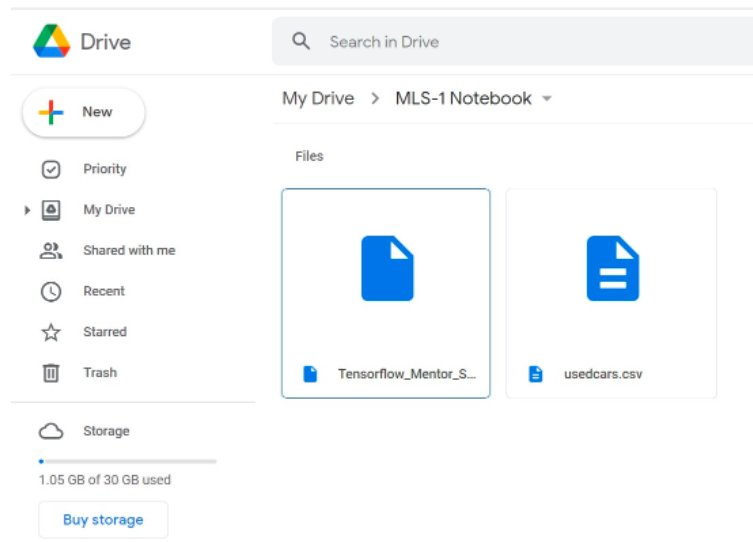
\includegraphics[height=2.0in]{googlecolab1}
		\caption{.}
		\label{fig:googlecolab1}
	\end{figure}

	\begin{figure}[h]
		\centering
		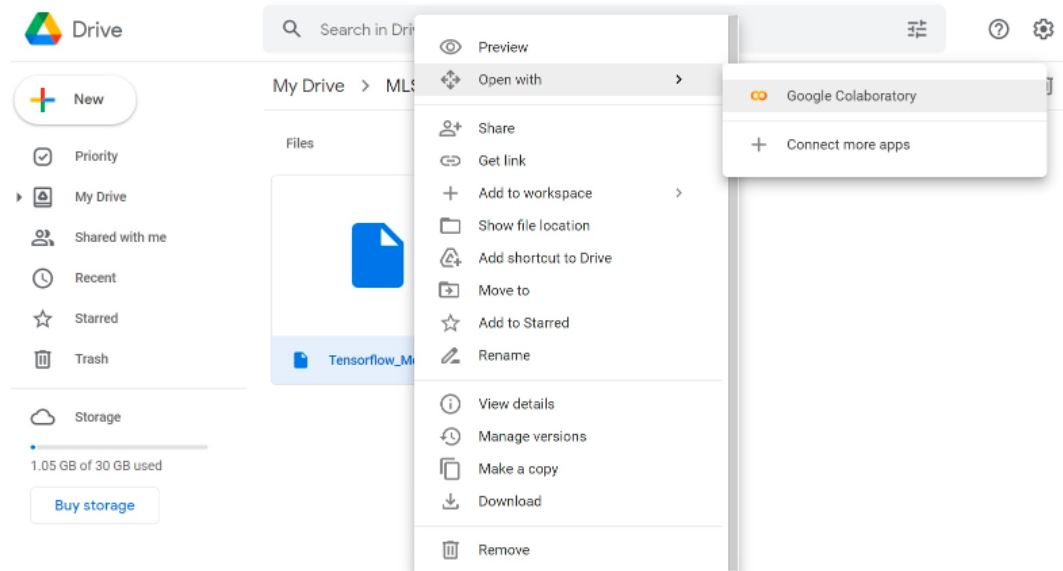
\includegraphics[height=2.0in]{googlecolab2}
		\caption{.}
		\label{fig:googlecolab2}
	\end{figure}

	\begin{figure}[h]
		\centering
		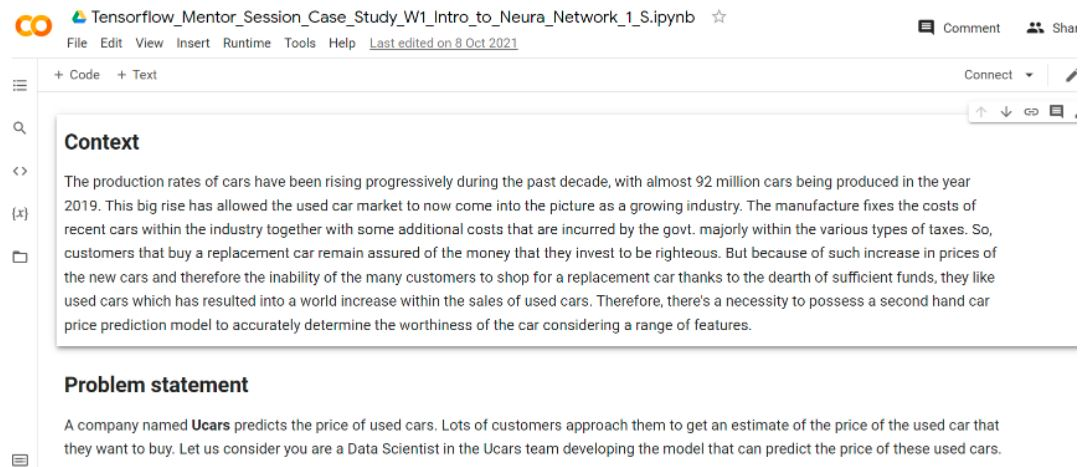
\includegraphics[height=2.0in]{googlecolab3}
		\caption{.}
		\label{fig:googlecolab3}
	\end{figure}

 	\begin{figure}[h]
		\centering
		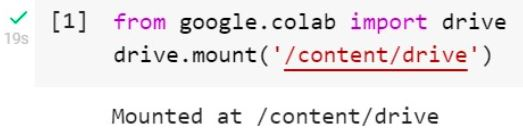
\includegraphics[height=0.75in]{googlecolab4}
		\caption{.}
		\label{fig:googlecolab4}
	\end{figure}
\clearpage{}

 	\begin{figure}[h]
		\centering
		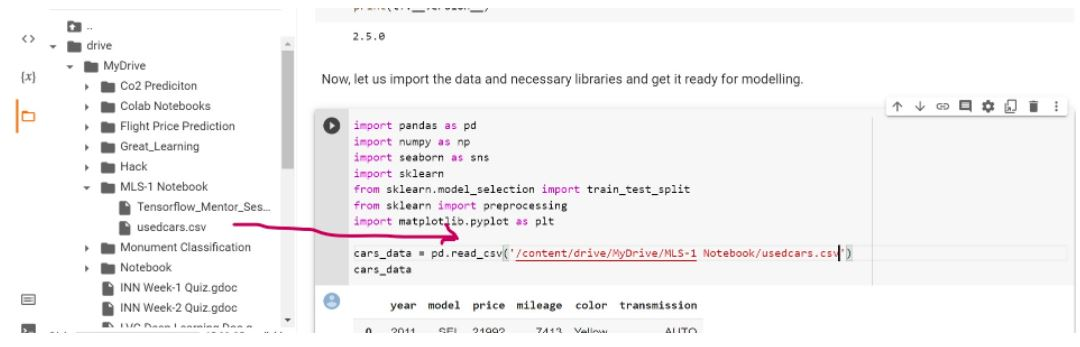
\includegraphics[height=1.75in]{googlecolab5}
		\caption{.}
		\label{fig:googlecolab5}
	\end{figure}


	\section{Deep Neural Network / Artificial Neural Network}

	\begin{bulletedlist}
		\item Deep Neural Network is an Artificial Neural Network with more than one hidden layer.
		\item An artificial Neural Network (ANN) is a model that employs a collection of artificial neurons to extract the patterns in the data that represent the relationship between independent and dependent variables.
		\item Artificial Neurons are based on the observed behavior of neurons in biological brains. A collection of artificial neurons mimic the behavior of biological neural networks.
		\item Just as brain uses a network of interconnected neurons to parallelize the processing of input signals to trigger a response, ANN also make use of interconnected neurons to work in parallel on input signals and give an output.
		\item In the initial days of the journey towards modern Deep Neural Networks, the research in artificial neuron and ANN were closely tied to the research in
neurology. The research in ANN borrowed ideas such as thresholds, linear summation, neuron firing or not etc from Neurology.
		\item However, the two fields today are de-linked and one does not need to know anything about biological neurons to work on ANN / DNN.
	\end{bulletedlist}

	\subsection{History}
Inspiration from neurology, see \figurename~\ref{fig:biologicalversusartificialneuron}.
 	\begin{figure}[h]
		\centering
		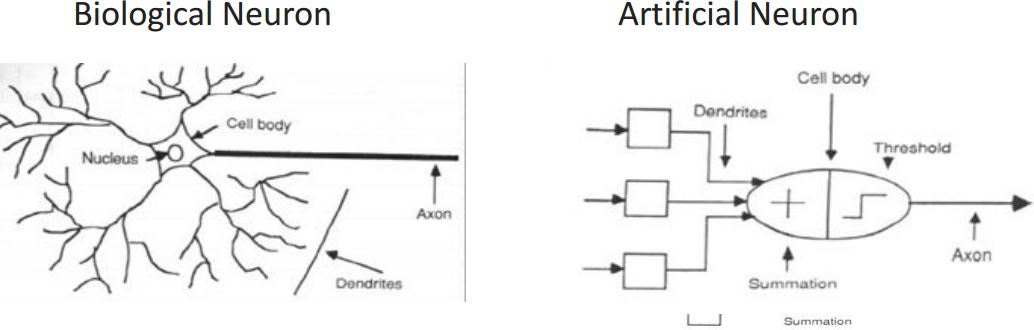
\includegraphics[height=1.75in]{biologicalversusartificialneuron}
		\caption{.}
		\label{fig:biologicalversusartificialneuron}
	\end{figure}

	\subsection{Boolean Gates and Artificial Neurons}

	\begin{bulletedlist}
		\item The objective of research in artificial neurons was to develop a computing system that could learn to do tasks on its own without instruction on how to do it.
		\item Most of the tasks that we do in our day-to-day life are classified. Hence, research was on to develop an artificial neuron that could classify.
		\item Since computing systems are based on Boolean gates which generated two classes, it was natural to check whether the artificial neurons can learn to mimic these gates such as the OR, AND gates.
	\end{bulletedlist}
See \figurename~\ref{fig:booleangates}.
 	\begin{figure}[h]
		\centering
		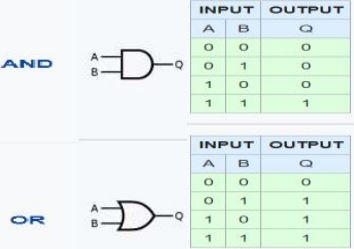
\includegraphics[height=1.75in]{booleangates}
		\caption{.}
		\label{fig:booleangates}
	\end{figure}

	\subsection{Warren McCulloch and Walter Pitts ``AND'', ``OR'' Neuron}

	\begin{bulletedlist}
		\item In McCulloch-Pitts neurons inputs and outputs are binary. The output is only one but inputs can be many.
		\item All inputs have same positive weights (not shown in the figure).
		\item The inputs multiplied with corresponding weights are summed up and the result sent to a step function.
		\item The threshold of the step function is fixed (for e.g. 1 for ``AND'' gate with two inputs each with weight 1).
		\item The threshold has to be modified for a gate, for e.g. ``AND'' gate depending on the number of inputs.  What would the threshold for the ``AND'' gate be if the number of inputs is x1, x2, x3?
		\item The McCulloch-Pitts model of a neuron is simple. However, this model is so simplistic that it only generates a binary output and also the weight and threshold values are
fixed.
	\end{bulletedlist}


{\bfseries AND Gate}
	\begin{code}[\codenumbering]{}
		\codeitemnonumber{w[1] = 1}
		\codeitemnonumber{w[0] = 1}
		\codeitemnonumber{training\_data = [}
		\stepcodelevel{}
			\codeitemnonumber{(array([0,0]), 0),}
			\codeitemnonumber{(array([0,1]), 0),}
			\codeitemnonumber{(array([1,0]), 0),}
			\codeitemnonumber{(array([1,1]), 1), ]}
 			\prevcodelevel{}
		\codeitemnonumber{\# Step function with threshold of >1. Anything below is 0}
		\codeitemnonumber{step\_function = lambda x: 0 if x < 1 else 1}
		\codeitemnonumber{w[1] = 1}
		\codeitemnonumber{w[0] = 1}
		\codeitemnonumber{for x, ? in training\_data:}
		\stepcodelevel{}
			\codeitemnonumber{result = dot(x, w)}
			\codeitemnonumber{print("\{\}: \{\} -> \{\}".format(x[:2], result, step\_function(result)))}
 			\prevcodelevel{}
	\end{code}

	\subsection{Rosenblatt Neuron Perceptron}
 	\begin{figure}[h]
		\centering
		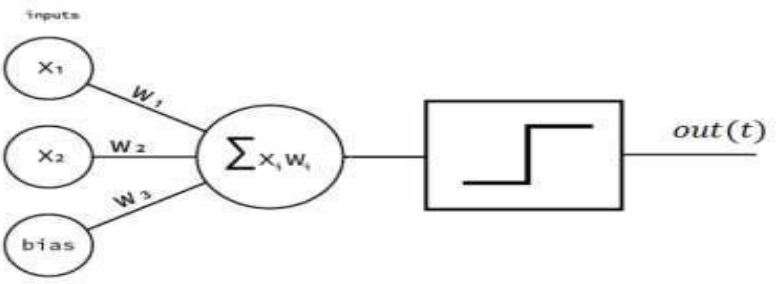
\includegraphics[height=1.25in]{rosenblattperceptron}
		\caption{.}
		\label{fig:rosenblattperceptron}
	\end{figure}
	\begin{bulletedlist}
		\item Uses weights for the inputs.  A concept borrowed from William Hebb's rule ``neurons that wire together, fire together.''
		\item Other than the inputs they also get a special ``bias'' input, which just has a value of 1.
		\item Incorrect outputs for a given input are captured as errors.
		\item A learning rule modifies the weight to correct errors in output.
		\item The neuron could behave like ``AND'' gate or ``OR'' gate with same threshold by adjusting weights.
		\item This neuron learns the patterns from the data. If the data is for ``AND'' gate, it learns to mimic ``AND'' gate.
		\item This concept of learning from data was a major improvement over McCulloch-Pitts neuron.
		\item Rosenblatt defined a perceptron as a simple mathematical model of biological neurons.
		\item It takes inputs as a set of binary values, every input is multiplied by a weight (synaptic strength to each nearby neuron).
		\item A threshold to evaluate the sum of weighted inputs against. Output a 1 (neuron firing) if the weighted sum is more than the threshold, else a zero (neuron not firing).
		\item Other than the inputs from sensors / neighboring neurons, they also get a special `bias' input, which just has a value of 1.
		\item The bias is like an intercept in a linear equation.  Useful in generating more functions with the same inputs.
		\item This was an improvement of the work of Warren McCulloch and Walter Pitts, McCulloch-Pitts neuron.
		\item McCulloch Pitts neuron had a fixed set of weights associated with inputs and as a result, did not have the ability to learn.
		\item They had no bias term either Rosenblatt's neuron was inspired by a rule coined by Donald Hebb (researcher studying biological neurons), according to which learning in brain is stored in form of changes to the strength of relationships between two connected neurons ``Neurons that fire together, wire together.''
		\item Rosenblatt's neuron can model the basic OR/AND/NOT functions (building blocks of computing systems).
		\item This was a big step towards the belief that making computers able to perform formal logical reasoning would essentially solve AI.
		\item Weights for the inputs are not the same, can be positive or negative.
		\item The output can be -1, 0, 1 unlike MCP neuron where the output is only 0 or 1.
		\item The neuron is associated with a learning rule that modifies the weight to ensure with the same threshold, the neuron can behave like an ``AND'' gate or ``OR'' gate with no need for any threshold modification.
		\item This neuron learns from the data. It has the intelligence to learn the pattern from the data.
	\end{bulletedlist}

Rosenblatt's Neuron Functioning
	\begin{numberedlist}
		\item Start with a random set of weights for all the input variables, and the bias.
		\item For the input data point, compute the output using the weights and the bias.
		\item If the calculated output does not match the expected output (from training data) modify the weights (The relation between weight adjustment and errors and a learning rate will make the learning possible. Learning is the process finding the right combination of weights that minimizes the errors in the training data set).
		\item Go to the next example in the training set and repeat steps j - k until the Perceptron makes no more mistakes.
	\end{numberedlist}

Perceptron Learning Algorithm
	\begin{numberedlist}
		\item Select random sample from training set as input. Draw the first random line (green) such that blue triangles lie above it and red circles ones below.
		\item If the classification is correct, do nothing. But the first time many blue triangles are on the wrong side!
		\item If the classification is incorrect, modify the weight vector w and shift the green line.
		\item Repeat this procedure until the entire training set is classified correctly.
		\item Howsoever times we run this algorithm, it will find a surface that separates the two classes.
		\item The Convergence theorem guarantees that when the classes are linearly separable in the training set, the perceptron will find that surface that separates the two classes correctly.
		\item The perceptron algorithm does not guarantee it will be able to separate the two classes correctly even when the classes are linearly separable.
		\item Why? Because it does not look for an optimal plane. It stops the moment it finds the separator plane (a.k.a dichotomizer).
		\item Since the planes are passing very close to the data points in the training set, they may not perform well in the test set where the distribution of the data will be different.
	\end{numberedlist}

 	\begin{figure}[h]
		\centering
		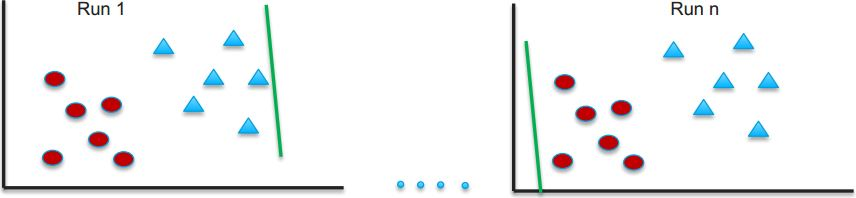
\includegraphics[height=1.25in]{perceptronlearningalgorithm1}
		\caption{}
		\label{fig:perceptronlearningalgorithm1}
	\end{figure}
 	\begin{figure}[h]
		\centering
		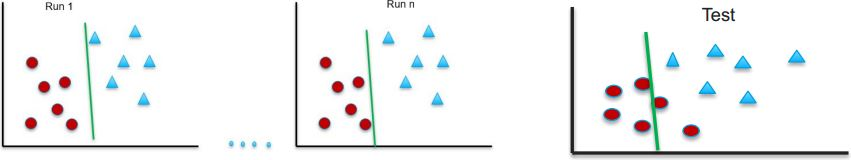
\includegraphics[height=1.25in]{perceptronlearningalgorithm2}
		\caption{}
		\label{fig:perceptronlearningalgorithm2}
	\end{figure}

	\begin{topcaptiontable}
        \centering
        \lecaption{}
        \label{tab:}
		\begin{tabular}{|p{0.5\qandatextwidth-2\tabcolsep}|p{0.5\qandatextwidth-2\tabcolsep}|} \hline
				\tablecolumnheadervlinesone{McCulloch-Pitts Neuron} & \tablecolumnheadervlinestwo{Rosenblatt's Perceptron} \\ \hline
				It has an input layer that acts like dendrites. &
				It has an Input layer that acts as dendrites. \\ \hline
				It has two parts, the first part, g is weighted addition of inputs. The weights are manually initialized and all have same weight. &
				It has two parts, first part is weighted addition Each input is multiplied with a weight (which is typically initialized with some random value) \\ \hline
				The weighted sum is passed through an activation function f which yields a 1 if threshold is crossed, else 0. &
				The sum is then passed through an activation function which yields a 1 if threshold is crossed. \\ \hline
				&
				The step function can be defined in such a way that output can range from -1 to +1. \\ \hline
				&
				It captured the error and had a logic built in to adjust the weights automatically to reduce the error. \\ \hline
		\end{tabular}
	\end{topcaptiontable}

	\subsection{Weakness of Perceptron}
	\begin{bulletedlist}
		\item Papert and Minsky demonstrated that the perceptron was incapable of handling some of the binary gates such as XOR**
		\item Given that it cannot represent all possible binary gates, it could not have been used for all possible computations hence the objective of computer based AI was a pipe dream!
		\item XOR is an example of distribution of classes not linearly separable in two dimensions but is easily separable in higher 3 dimensional space. Ref: http://www.mind.ilstu.edu/curriculum/artificial\_neural\_net/xor\_problem\_and\_solution.php
		\item It was subsequently demonstrated that instead of making a neuron intelligent, a network of neurons can be used to do what a single neuron could not
		\item This was the birth of a Artificial Neural Network
	\end{bulletedlist}

	\section{Artificial Neural Networks}

	\begin{bulletedlist}
		\item Perceptrons were replaced with artificial neuron which not only had a weighted summation operation but also included a non-linearity function.
		\item Multitude of such neurons working together could solve those problems where individual perceptrons failed.
		\item Multiple neurons in a single layer is akin to transforming data from lower dimensions to higher dimensions! (Cover's theorem in action).
		\item Kolgomorov theorem* states that any continuous function f(x1,x2,...,xn) defined on [0,1] with n>2 can be expressed in form of two carefully chosen functions
		\item Looks similar to layer of neurons with non-linear function g acting on summation of weighted inputs!  No wonder NeuralNets form basis of complex processing.
		\item The processing element of an ANN is called a node, representing the artificial neuron.  Each ANN is composed of a collection of nodes grouped in layers. A typical structure is shown The initial layer is the input layer and the last layer is the output layer.  In between, we have the hidden layers.
	\end{bulletedlist}
 	\begin{figure}[h]
		\centering
		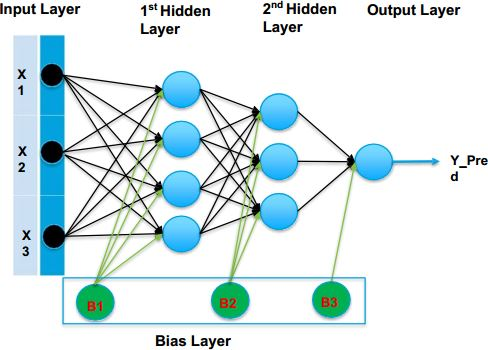
\includegraphics[height=2.25in]{artificialneuralnetwork}
		\caption{}
		\label{fig:artificialneuralnetwork}
	\end{figure}

	\subsection{Fully Connected Artificial Neural Network}
	\begin{numberedlist}
		\item The input layer is passive, does no processing, only holds the input data to supply it to he first hidden layer (\figurename~\ref{fig:artificialneuralnetworkfullyconnected1}).
		\item Each node in the first hidden layer, takes all input attributes, multiplies with the corresponding weights, adds bias and the output is transformed using non-linear
function (\figurename~\ref{fig:artificialneuralnetworkfullyconnected2}).
		\item The weights for a given hidden node is pre-fixed and all the nodes in the hidden layer have their own weights.
		\item The output of each node is fed to output layer nodes or another set of hidden nodes in another hidden layer.
		\item The output value of each hidden node is sent to each output node in the output layer (\figurename{}s~\ref{fig:artificialneuralnetworkfullyconnected3},~\ref{fig:artificialneuralnetworkfullyconnected4}).
		\item In a binary output ANN, the output node acts like a perceptron classifying the input into one of the two classes (\figurename~\ref{fig:artificialneuralnetworkfullyconnected5}).
		\item Examples of such ANN applications would be to detect fraudulent transaction, whether a customer will buy a product given the attributes etc.
		\item ANN can also be used for multi-class classification problems such as digit recognition. In fact, it is often used for multi-class classification.
		\item The processing elements of a ANN is called a node, representing the artificial neuron. Each ANN is composed of a collection of nodes grouped in layers.  A typical structure is shown.  The initial layer is the input layer and the last layer is the output layer.  In between we have the hidden layers (\figurename~\ref{fig:artificialneuralnetworkfullyconnected6}).
		\item Mathematical foundations for artificial neural networks.
		\begin{numberedlist}
			\item Kolmogorov theorem - any continuous function f defined on n-dimensional cube is representable by sums and superpositions of continuous functions of only one variable.
			\item Cover's theorem - states that given a set of training data that is not linearly separable, one can with high probability transform it into a training set that is linearly separable by projecting it into a higher-dimensional space via some non-linear transformation.
		\end{numberedlist}
		\item A given node will fire and feed a signal to subsequent nodes in next layer only if the non-linear function it implements reaches a threshold.
		\item In ANN use of Sigmoid function is more common than step function (\figurename~\ref{fig:artificialneuralnetworkfullyconnected7}).
	\end{numberedlist}

 	\begin{figure}[h]
		\centering
		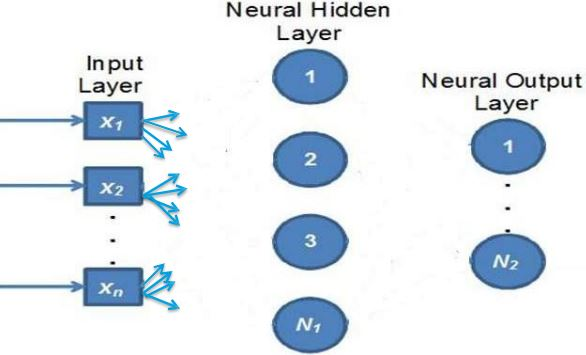
\includegraphics[height=2.0in]{artificialneuralnetworkfullyconnected1}
		\caption{}
		\label{fig:artificialneuralnetworkfullyconnected1}
	\end{figure}
 	\begin{figure}[h]
		\centering
		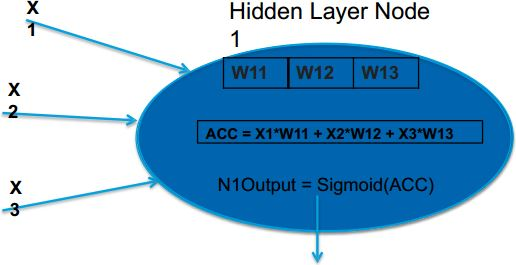
\includegraphics[height=2.0in]{artificialneuralnetworkfullyconnected2}
		\caption{}
		\label{fig:artificialneuralnetworkfullyconnected2}
	\end{figure}
 	\begin{figure}[h]
		\centering
		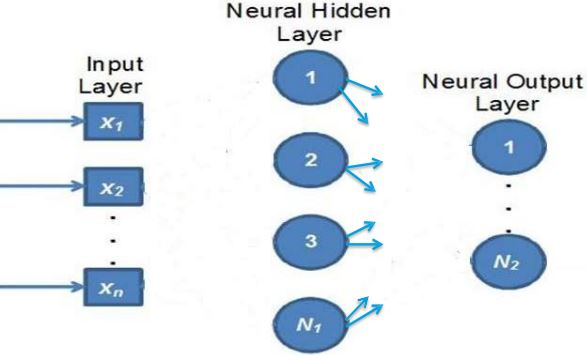
\includegraphics[height=2.0in]{artificialneuralnetworkfullyconnected3}
		\caption{}
		\label{fig:artificialneuralnetworkfullyconnected3}
	\end{figure}
 	\begin{figure}[h]
		\centering
		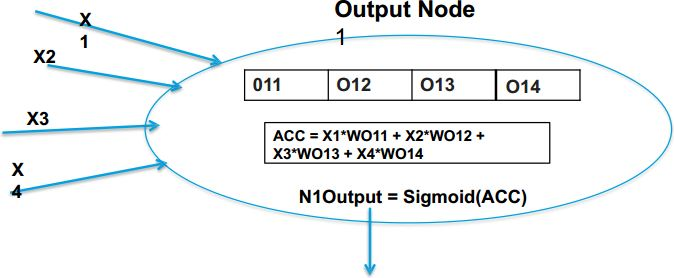
\includegraphics[height=2.0in]{artificialneuralnetworkfullyconnected4}
		\caption{}
		\label{fig:artificialneuralnetworkfullyconnected4}
	\end{figure}
 	\begin{figure}[h]
		\centering
		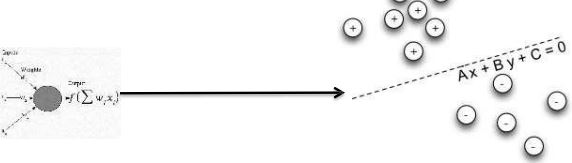
\includegraphics[height=1.5in]{artificialneuralnetworkfullyconnected5}
		\caption{}
		\label{fig:artificialneuralnetworkfullyconnected5}
	\end{figure}
 	\begin{figure}[h]
		\centering
		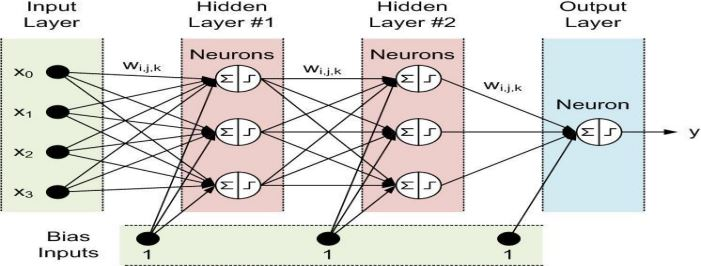
\includegraphics[height=1.5in]{artificialneuralnetworkfullyconnected6}
		\caption{}
		\label{fig:artificialneuralnetworkfullyconnected6}
	\end{figure}

	\subsection{Application of Artificial Neural Networks}

	\begin{bulletedlist}
		\item We can have a ANN with multiple output nodes where a given output node may or may not get triggered given the input and the weights.
		\item The weights required to make a neural network carry out a particular task are found by a learning algorithm, together with  examples of how the system  should operate.
		\item The examples in vehicle identification could be a large hadoop file of several millions sample segments such as bicycle, motorcycle, car, bus etc.
		\item The learning algorithms calculate the appropriate weights for each classification for all nodes at all the levels in the network.
		\item If we consider each input as a dimension then ANN labels different regions in the n-dimensional space. In our example one region is cars, other region is bicycle.
	\end{bulletedlist}

	\subsection{Classification}
	\begin{bulletedlist}
		\item Classification always refers to a predictive modeling problem, where the input data is classified into one of the predefined existing classes. In Supervised machine learning the output labels are always known. For example: predicting a patient having cancer or not is an example of binary classification problem.
		\item We have come across many Machine Learning algorithms used for classification but Neural networks can mainly be used when we have many output classes or labels and we have high amount of data for the model.
		\item ANN has many advantages when used for classification but it even has some disadvantages like higher computational costs and longer training time.
	\end{bulletedlist}

 	\begin{figure}[h]
		\centering
		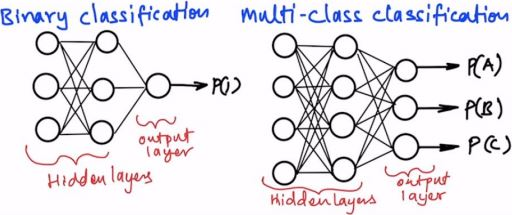
\includegraphics[height=1.5in]{artificialneuralnetworkclassification}
		\caption{}
		\label{fig:artificialneuralnetworkclassification}
	\end{figure}

	\subsection{Regression}
	\begin{bulletedlist}
		\item Regression always refers to a predictive modeling problem, where the output values are predicted as a continuous value as a function of inputs.
		\item Regression models mostly work well when the regression equations fits well on the data.  And using ANN is similar to classification but we need to replace the final layer used in the classification model with a fully connected layer with a single node with a single activation function.
	\end{bulletedlist}
 	\begin{figure}[h]
		\centering
		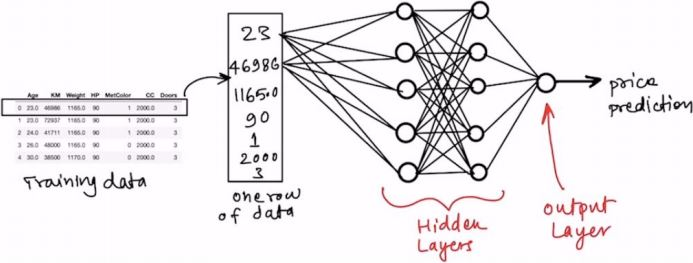
\includegraphics[height=1.5in]{artificialneuralnetworkregression}
		\caption{}
		\label{fig:artificialneuralnetworkregression}
	\end{figure}

	\section{Multi-Layer Perceptron}

	\begin{bulletedlist}
		\item The operation of one perceptron with sigmoid as the activation function is same as the logistic regression algorithm.
	\end{bulletedlist}

	\section{MNIST Dataset}
	\begin{bulletedlist}
		\item Numbers as images of size 28x28 pixels and labeled.
		\item Activation functions should be non-linear.  If all activation functions are linear, the neural network is equivalent to linear regression.
		\item Networks often find a local minimum not a global.  The global solution is often over fit (specific to the particular data set).  The local minimums are often more robust (not over fit).
	\end{bulletedlist}


	\section{Activation Functions}

	\begin{bulletedlist}
		\item Artificial neuron works in three steps.
		\begin{numberedlist}
			\item First it multiplies the input signals with corresponding weights.
			\item Second, adds the weighted signals.
			\item Third, converts the result to another value using a mathematical transformation function.
		\end{numberedlist}
		\item For the third step, there are multiple mathematical functions available but all together are called the activation function.
		\item The purpose of the activation function is to act like a switch for the neuron. Should the neuron fire or not.
		\item The activation function is critical to the overall functioning of the neural network. Without it, the whole neural network will mathematically become equivalent to one single neuron!
		\item Activation function is one of the critical component that gives the neural networks ability to deal with complex problems.
		\item Let us take a fully connected neural network. Every neuron in every layer takes multiple inputs.
		\item The inputs are weighted and summed up at each neuron
		\item The nodes in the second layer are simply scaling up the output of neurons in previous layer.
		\item For e.g.\ the neuron G takes as input weight sums from D, E, and F, G's output is scaled version of output of D, E, and F
		\item See \equationname~\ref{eq:neuronweights}
		\item Thus this part of the network is like a single neuron with weights of 8, 6, 3
		\item Same argument holds for other neurons.
		\item Thus the entire neural network collapses to on neuron!
		\item A single neuron is not capable of doing much.
	\end{bulletedlist}


	\begin{align}
		\begin{split}
		 G_{out}	& = 3D -2E + 1F	\\
				& = 3(1A + 2B + 3C) - 2(-3A + 2B -1C) + 1(2A+4B-2C)	\\
				& = 8A + 6B + 3C
		\end{split}
		\label{eq:neuronweights}
	\end{align}

 	\begin{figure}[h]
		\centering
		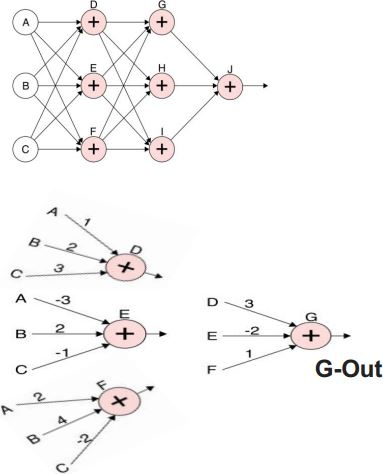
\includegraphics[height=2.5in]{activationfunctions1}
		\caption{}
		\label{fig:activationfunctions1}
	\end{figure}

	\begin{bulletedlist}
		\item The activation functions are a mathematical transformations that prevent the network from collapsing to a single neuron.
		\item The collapse can happen when the neurons do simple addition and multiplications of the inputs. These are called linear operations. Thus linear operations collapse the network
		\item All activations functions are nonlinear transformers for exactly the same reason. This non-linear transformation not only prevents collapse, it also empowers the network to do complex tasks because each neuron does something in the network totality.

		\item Types of non-linear activation functions include:
		\begin{bulletedlist}
			\item Piecewise linear functions.
			\begin{bulletedlist}
				\item Step function.
				\item ReLU - Rectified Linear Units
				\item Leaky ReLU
				\item Parametric ReLU
				\item Shifted ReLU
			\end{bulletedlist}
			\item Smooth functions
			\begin{bulletedlist}
				\item Smooth ReLU / Exponential ReLU
				\item Sigmoid / Logistic functions
				\item Hyperbolic Tangent (tanh)
				\item Swish (combination of Sigmoid and ReLU)
			\end{bulletedlist}
		\end{bulletedlist}
	\end{bulletedlist}

 	\begin{figure}[h]
		\centering
		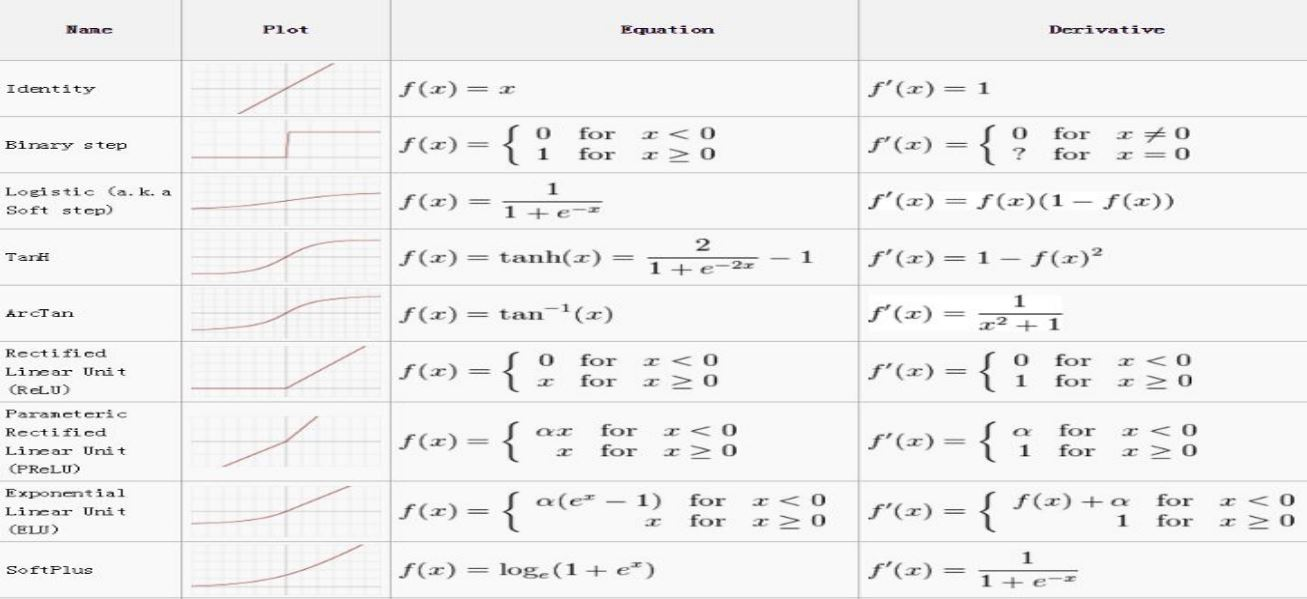
\includegraphics[width=\textwidth,height=4.5in]{activationfunctions2}
		\caption{}
		\label{fig:activationfunctions2}
	\end{figure}


	\begin{bulletedlist}
		\item For both large positive and negative input values, sigmoid doesn't change much with change of input.The problem with sigmoid is (near) zero gradient on both extremes
		\item ReLU has a constant gradient for almost half of the inputs
		\item But, ReLU cannot give a meaningful final output
		\item Sigmoid gives binary classification output
		\item Tanh can also do that provided the desired output is in {-1, +1}
		\item Softmax generalizes sigmoid to n-array classification
		\item Linear is used for regression
		\item ReLU is only used in internal nodes (non-output)
	\end{bulletedlist}



 	\begin{figure}[h]
		\begin{minipage}[t]{0.48\textwidth}
			\centering
			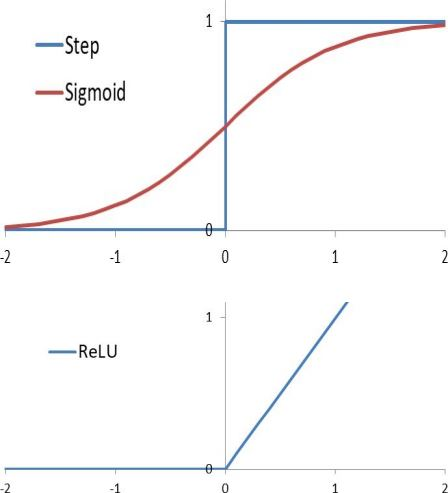
\includegraphics[height=2in]{activationfunctionscomparison1}
		\end{minipage}
		\hfill
		\begin{minipage}[t]{0.48\textwidth}
			\centering
			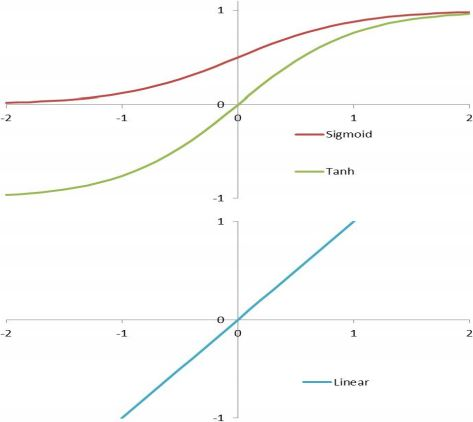
\includegraphics[height=2in]{activationfunctionscomparison2}
		\end{minipage}
		\caption{}
		\label{fig:activationfunctionscomparison}
	\end{figure}


	\subsection{ReLU vs Simple Linear Activation Function}
	\begin{bulletedlist}
		\item Half range of ReLU (default ReLU) is a simple linear transformation of the form $y = mx$ (as long as $mx +c > 0$),
for $mx + c <=0 y = 0$
		\item If half of the input is transformed using linear model, then why does not ReLU network collapse to perceptron?
To understand this let us look at the dummy network in \figurename~\ref{fig:reluversuslineaar} which has no nonlinear transformation.
		\item When we replace all the neurons in the network with the neuron shown above with ReLU, Gout will be 0 if $3D
-2E + 1F < = 0$ and $3D - 2E + 1F$ will be same as Gout only when $3D -2E + 1F is > 0$.
		\item Thus, Gout cannot be generalized as $3D -2E + 1F$. Same goes for $D0$, $E0$, and $F0$. Hence the neuron does not
become an equivalent of a perceptron.
	\end{bulletedlist}

 	\begin{figure}[h]
		\centering
		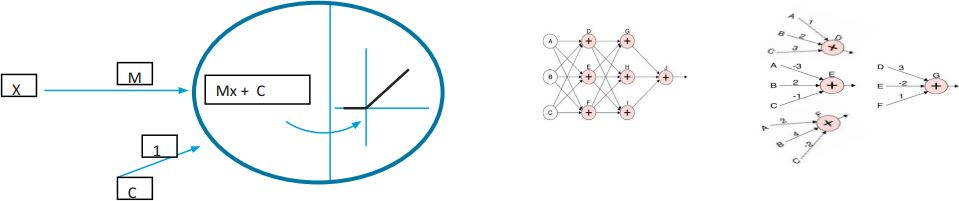
\includegraphics[width=\textwidth]{reluversuslineaar}
		\caption{}
		\label{fig:reluversuslineaar}
	\end{figure}


	\subsection{Step Function}
	\begin{bulletedlist}
		\item Step function divides the input space into two halves, 0 and 1.
		\item In a single neuron, step function is a linear binary classifier.
		\item The weights and biases determine where the step will be in n-dimensions.
		\item But, as we shall see later, it gives little information about how to change the weights if we make a mistake.
		\item So, we need a smoother version of a step function.
	\end{bulletedlist}

	\subsection{Sigmoid Function}
	\begin{bulletedlist}
		\item
	\end{bulletedlist}

	\subsection{Softmax Function}
	\begin{bulletedlist}
		\item A kind of operation applied at the output neurons of a classifier network.
		\item Used only when we have two or more output neurons and is applied simultaneously to all the output neurons.
		\item Turns raw numbers coming out of the pen-ultimate layer into probability values in the output layer
		\item Suppose output layer neurons emit (Op1, Op2, Opn). The raw numbers may not make much sense. We convert that into probabilities using Softmax which becomes more meaningful. For e.g. input belongs to cycle is 30 times more likely than sailboat, 13 times more probable than car.
	\end{bulletedlist}

 	\begin{figure}[h]
		\centering
		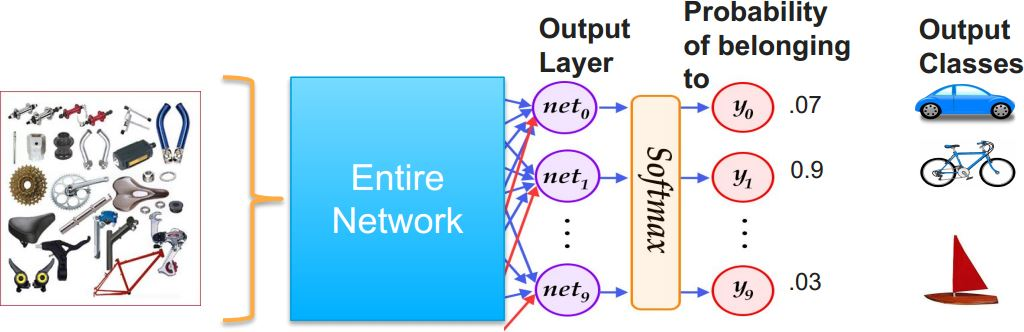
\includegraphics[width=\textwidth]{softmax}
		\caption{}
		\label{fig:softmax}
	\end{figure}


	\subsection{Cover's Theorem}

 	\begin{figure}[h]
		\centering
		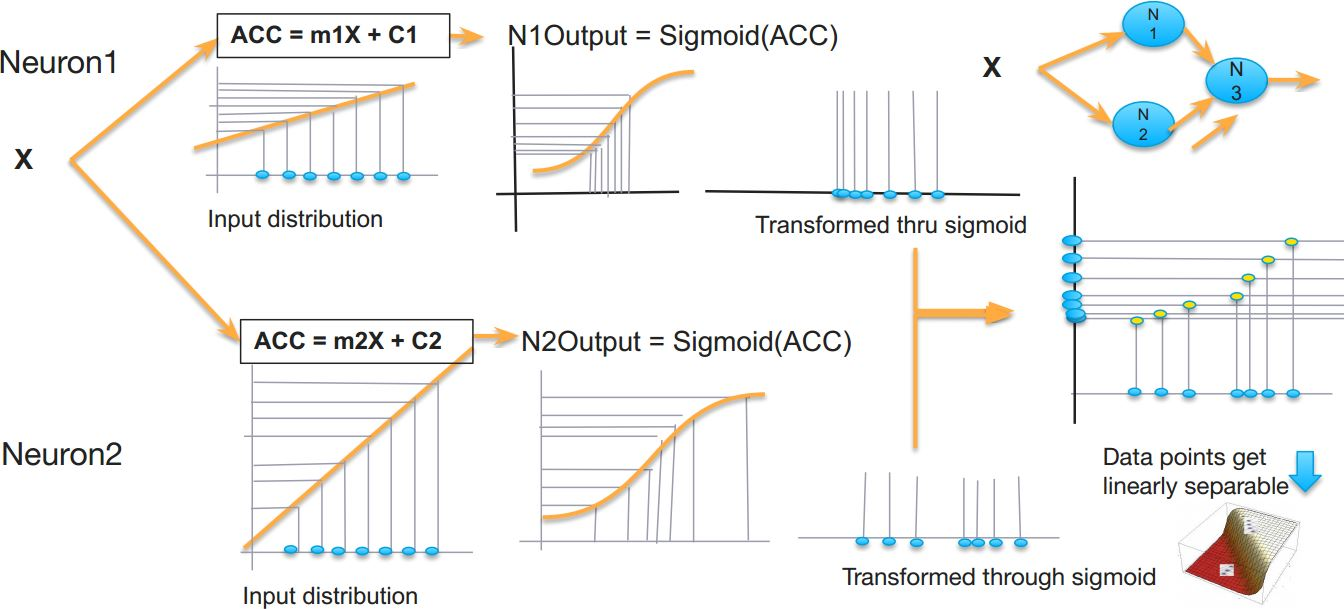
\includegraphics[width=\textwidth]{activationfunctionscoverstheorem1}
		\caption{}
		\label{fig:activationfunctionscoverstheorem1}
	\end{figure}
 	\begin{figure}[h]
		\centering
		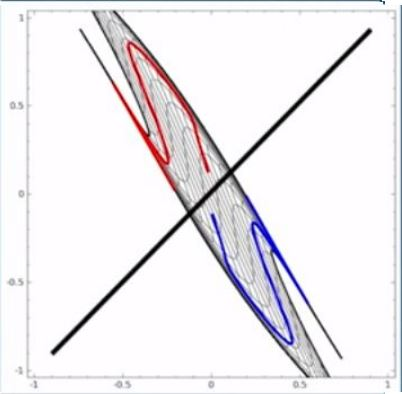
\includegraphics[width=2in]{activationfunctionscoverstheorem2}
		\caption{Neurons stretch the features pace through non-linear functions and achieve Cover's theorem.}
		\label{fig:activationfunctionscoverstheorem2}
	\end{figure}

	\section{Where to Use}
	\subsection{Output}
	\subsubsection{Binary Classification}
For binary classification problems:
	\begin{bulletedlist}
		\item Sigmoid (0 and 1)
		\item Tanh (-1 and 1)
	\end{bulletedlist}

	\subsubsection{Regression}
For regression problems:
	\begin{bulletedlist}
		\item Linear
	\end{bulletedlist}

	\subsubsection{Multi-class Classification}

Use multiple output nodes, one for each possible output.

Activation function:
	\begin{bulletedlist}
		\item Softmax
	\end{bulletedlist}

Use Softmax which takes input from all nodes and creates normalized output.  Uses an exponential function to do the normalization.

	\subsection{Hidden Layers}
	\begin{bulletedlist}
		\item Sigmoid
		\item Tanh
		\item ReLU
		\item Leaky ReLU
	\end{bulletedlist}


	\section{Deep Learning Notations}

	\section{Forward Propagation and Bias}
	\begin{bulletedlist}
		\item The directed acyclic path taken by input data from input layer to get transformed using non-linear functions into final network level outputs.
		\item Input data is propagated forward from the input layer to hidden layer till it reaches final layer where predictions are emitted.
		\item At every layer, data gets transformed non-linearly in every neuron.
		\item There may be multiple hidden layers with multiple neurons in each layer.
		\item The last layer is the output layer which may have a Softmax function (if the network is a multi class classifier).
		\item Forward prop steps:
		\begin{numberedlist}
			\item Calculate the weighted input to the hidden layer by multiplying $X$ by the hidden weight $Wh$.
			\item Apply the activation function and pass the result to the final layer.
			\item At output layer, repeat step 2 replacing $X$ by the hidden layer's output.
		\end{numberedlist}
	\end{bulletedlist}
 	\begin{figure}[h]
		\centering
		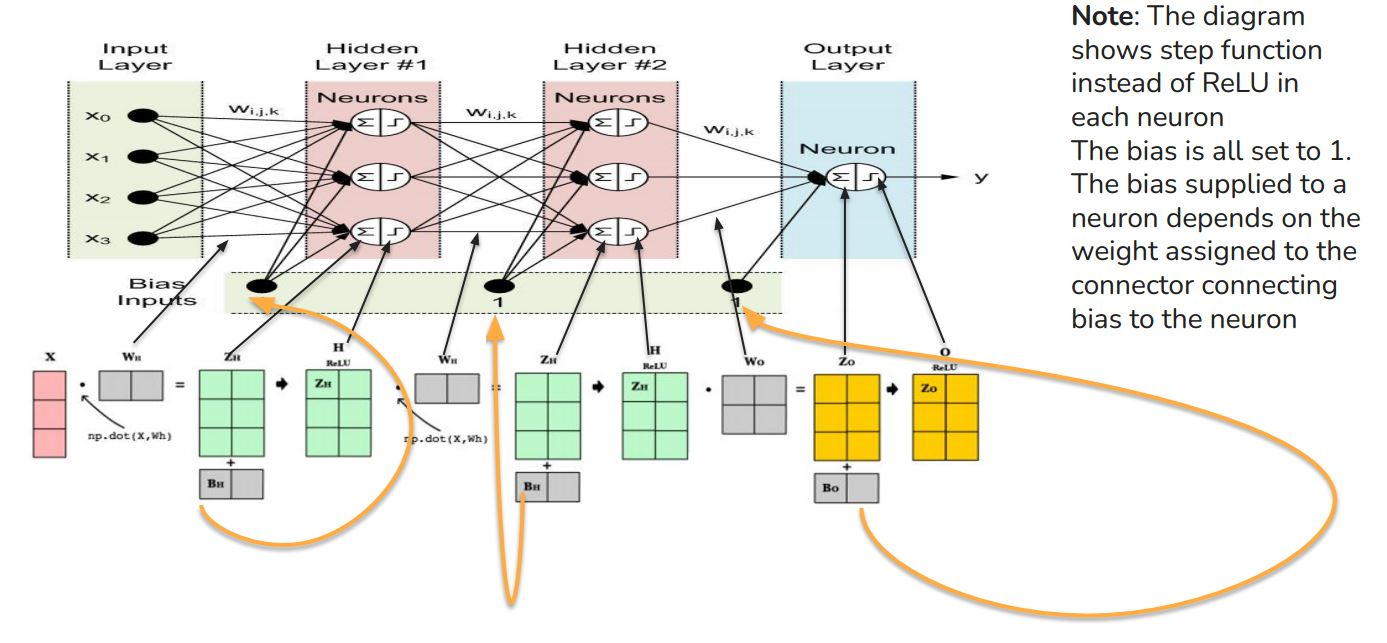
\includegraphics[height=2in]{forwardpropagation}
		\caption{}
		\label{fig:forwardpropagation}
	\end{figure}

	\subsection{Bias Term}
	\begin{bulletedlist}
		\item Every neuron in the hidden layers are associated with a bias term. The bias term help us to control the firing threshold in each neuron.
		\item It acts like the intercept in a linear equation ($y = sum(mx) + c$). If sum($mx$) is not crossing the x`threshold but the neuron needs to fire.
		\item Bias will be adjusted to lower that neuron's threshold to make it fire! Network learns richer set of patterns using bias.
		\item The bias term is also considered as input though it does not come from data.
	\end{bulletedlist}
 	\begin{figure}[h]
		\centering
		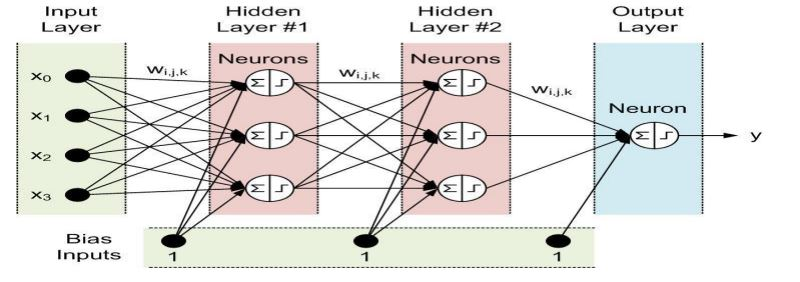
\includegraphics[height=2in]{fowardpropagationbiasterm}
		\caption{}
		\label{fig:fowardpropagationbiasterm}
	\end{figure}


	\section{Loss Function}
Calculates the error of the output to the actual.
	\begin{bulletedlist}
		\item Loss trends opposite of accuracy.
		\begin{bulletedlist}
			\item Loss is low when accuracy is high.
			\item Loss is zero for perfect accuracy (by convention).
			\item Loss is high when accuracy is low.
		\end{bulletedlist}
		\item Loss is a function of actual and desired output.
		\item Minimizing the loss function with respect to parameters leads to good parameters.
	\end{bulletedlist}

Properties of a good loss function:
	\begin{bulletedlist}
		\item Minimum value for perfect accuracy.
		\begin{bulletedlist}
			\item Usually zero.
			\item Note: low loss on training does not guarantee low loss on validation or testing.
		\end{bulletedlist}
		\item Varies smoothly with input.
		\item Varies smoothly with parameters.
		\item Good to be convex in parameters (but is usually not).
		\begin{bulletedlist}
			\item Like a paraboloid.
		\end{bulletedlist}
	\end{bulletedlist}

Loss and accuracy:
	\begin{bulletedlist}
		\item Training accuracy saturates to a maximum.
		\item Training loss saturates to a minimum.
		\item Loss is a measure of error.
	\end{bulletedlist}
 	\begin{figure}[h]
		\centering
		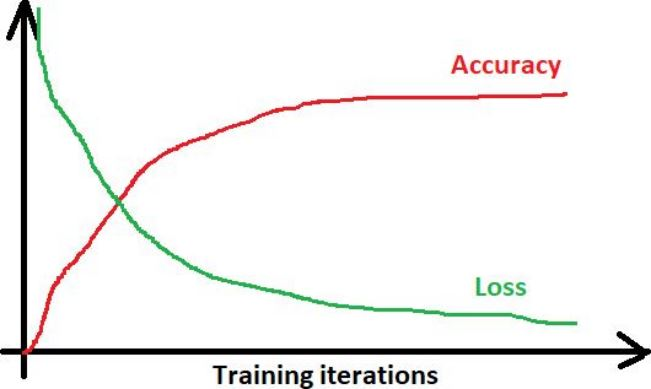
\includegraphics[height=2in]{lossandaccracy}
		\caption{}
		\label{fig:lossandaccracy}
	\end{figure}
 	\begin{figure}[h]
		\centering
		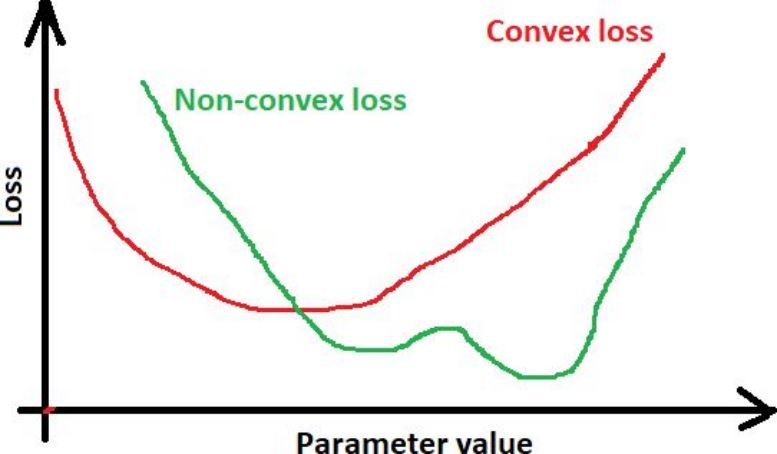
\includegraphics[height=2in]{lossconvexversusnonconvex}
		\caption{}
		\label{fig:lossconvexversusnonconvex}
	\end{figure}
 	\begin{figure}[h]
		\centering
		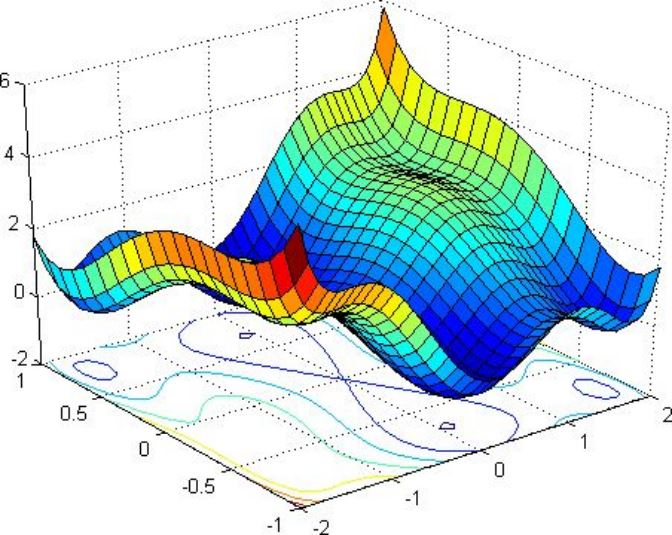
\includegraphics[height=2in]{lossnonconvexlocalminimum}
		\caption{}
		\label{fig:lossnonconvexlocalminimum}
	\end{figure}



Choice of loss function depends on:
	\begin{bulletedlist}
		\item Desired output type: continuous or categorical?
		\item Predicted output type: continuous or categorical?
		\item Goal: supervised or unsupervised?
		\item Loss function over a set is the average of loss over each sample in the set.
		\item Loss function over the validation set is the most important thing to monitor during training.
		\item High training loss means under-fitting.
		\item Large gap between training and validation losses means over-fitting.
	\end{bulletedlist}

Examples of loss functions:
	\begin{bulletedlist}
		\item Regression with continuous output
		\begin{bulletedlist}
			\item Mean square error (MSE), log MSE, mean absolute error
		\end{bulletedlist}
		\item Classification with probabilistic output
		\begin{bulletedlist}
			\item Cross entropy (negative log likelihood), hinge loss
		\end{bulletedlist}
		\item Similarity between vectors or clustering
		\begin{bulletedlist}
			\item Euclidean distance, cosine
		\end{bulletedlist}
	\end{bulletedlist}

 	\begin{figure}[h]
		\centering
		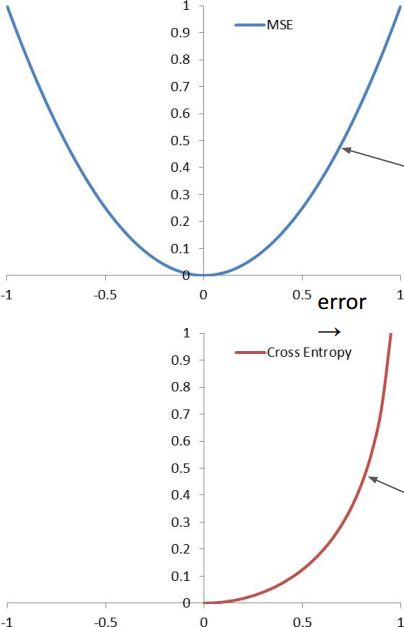
\includegraphics[height=3.5in]{lossfunctions1}
		\caption{There are positive and negative errors in classification and MSE is the most common loss function.  There is a probability of correct class
in classification, for which cross entropy is the most common loss function.}
		\label{fig:lossfunctions1}
	\end{figure}
 	\begin{figure}[h]
		\centering
		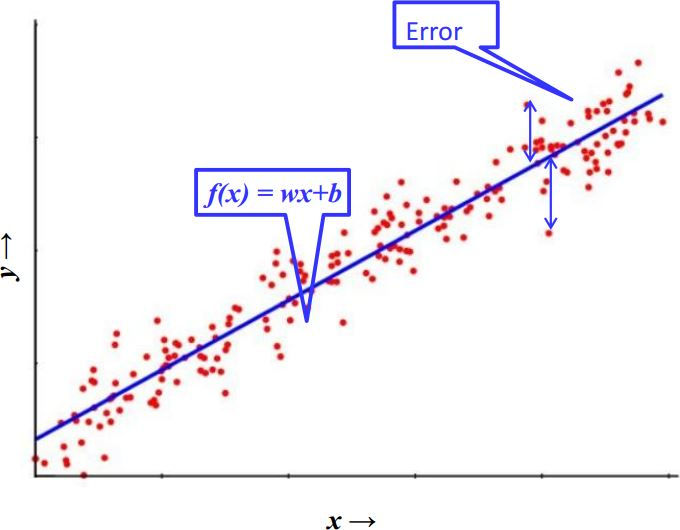
\includegraphics[height=2.5in]{lossmseforregression}
		\caption{Mean square error.}
		\label{fig:lossmseforregression}
	\end{figure}
 	\begin{figure}[h]
		\centering
		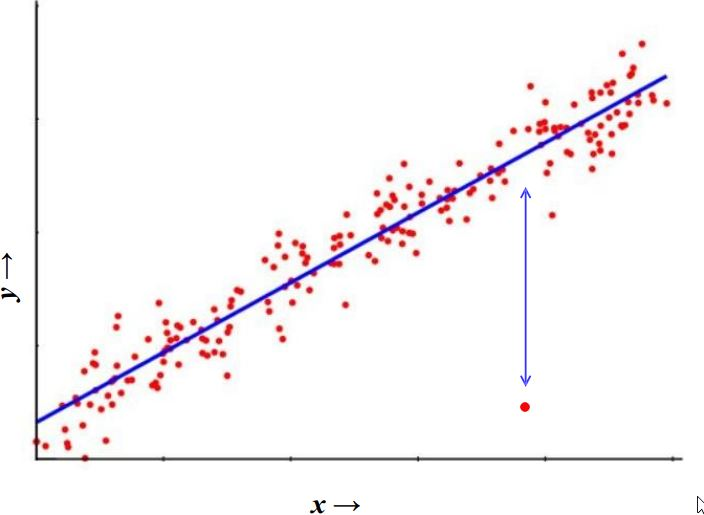
\includegraphics[height=2.5in]{lossmaeforregression}
		\caption{Mean absolute error.}
		\label{fig:lossmaeforregression}
	\end{figure}


All of the following are considered the same:
	\begin{bulletedlist}
		\item L2 loss function
		\item mean square error
		\item sum of squares error
	\end{bulletedlist}

Mean square error is shown in \equationname~\ref{eq:meansquareerror}.  Mean absolute error is shown in \equationname~\ref{eq:meanabsoluteerror}.
	\begin{equation}
		\frac{1}{n} \sum_i \left( y_i - \hat{y}_i \right)^2
		\label{eq:meansquareerror}
	\end{equation}
	\begin{equation}
		\frac{1}{n} \sum_i \left| y_i - \hat{y}_i \right|
		\label{eq:meanabsoluteerror}
	\end{equation}	
	\begin{mathwhere}
		\mathdefitem{n}{number of data points;}
		\mathdefitem{y_i}{observed values;}
		\mathdefitem{\hat{y}_i}{predicted values.}
	\end{mathwhere}

 	\begin{figure}[h]
		\centering
		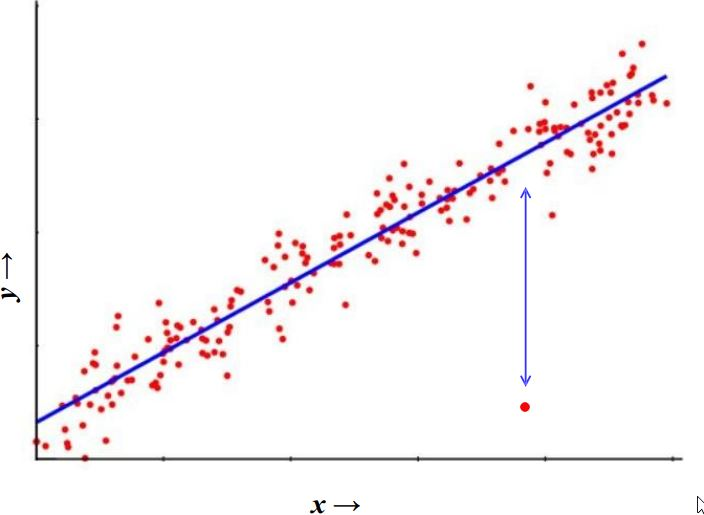
\includegraphics[height=2.5in]{lossmaeforregression}
		\caption{Mean absolute error.}
		\label{fig:lossmaeforregression}
	\end{figure}

	\subsection{Classification}
Cross entropy


	\section{Local Optimum and Saddle Point}

	\section{Back Propagation}
Back propagation uses the chain rule to make for more efficient calculations of the gradients.

	\begin{bulletedlist}
		\item Back propagation is the process of learning that the neural network employs to re-calibrate the weights and bias at every layer and every node to minimize the error in the output layer
		\item During the first pass of forward propagation, the weights and bias are random number. The random numbers are generated within a small range say 0-1
		\item Needless to say, the output of the first iteration is almost always incorrect. The difference between actual value / class and predicted value / class is the error
		\item All the nodes in all the preceding layers have contributed to the error and hence need to get their share of the error and correct their weights
		\item This process of allocating proportion of the error to all the nodes in the previous layer is back propagation
		\item The goal of back propagation is to adjust weights and bias in proportion to the error contribution and in iterative process identify the optimal combination of weights
		\item At each layer, at each node, gradient descent algorithm is applied to adjust the weights
	\end{bulletedlist}

 	\begin{figure}[h]
		\centering
		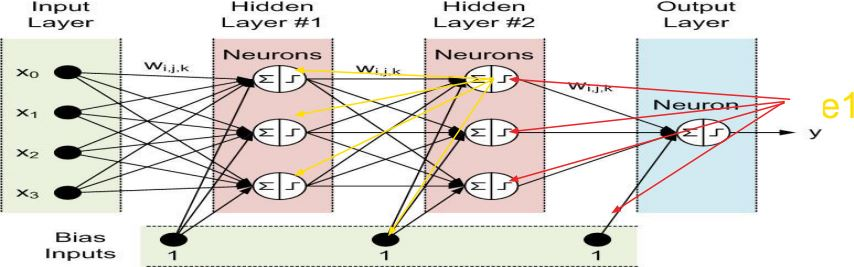
\includegraphics[height=1.75in]{backpropagation}
		\caption{Back propagation.}
		\label{fig:backpropagation}
	\end{figure}

	\begin{bulletedlist}
		\item Error in output node shown as e1, is contributed by node 1, 2, and 3 of layer 2 through weights w(3,1), w(3,2), w(3,3).
		\item Proportionate error is assigned back to node 1 of hidden layer 2 is (w(3,1) / w(3,1) + w(3,2) + w(3,3)) * e1.
		\item The error assigned to node 1 of hidden layer 2 is proportionately sent back to hidden layer 1 neurons.
		\item All the nodes in all the layers re-adjust the input weights and bias to address the assigned error (for this they use gradient descent).
		\item The input layer is not neurons, they are like input parameters to a function and hence have no errors.
	\end{bulletedlist}


	\section{Gradient Descent}

	\begin{bulletedlist}
		\item Gradient descent minimizes the loss function.
		\item At every point, compute:
		\begin{bulletedlist}
			\item Loss (scalar): $l_i(w)$
			\item Gradient of loss with respect to weights (vector): $\nabla l_i(w)$
			\item Take a step towards negative gradient:
		\end{bulletedlist}
	\end{bulletedlist}

Role of step size and learning rate
	\begin{bulletedlist}
		\item Tale of two loss functions
		\begin{bulletedlist}
			\item Same value
			\item Same gradient (first derivative), but
			\item Different Hessian (second derivative)
			\item Different step sizes needed
		\end{bulletedlist}
		\item Success is not guaranteed
	\end{bulletedlist}

	\begin{bulletedlist}
		\item The perfect step size is impossible to guess. Goldilocks finds the perfect balance only in a fairy tale
		\item The step size is decided by learning rate $\eta$ and the gradient
	\end{bulletedlist}

	\begin{bulletedlist}
		\item Vanilla gradient descent: use samples in a fixed sequence: %$w_{n+1} = w_n	 - \eta \left( \sum_{i=1}^n l_i(w) \right)$
		\item Stochastic gradient descent: Choose a random sample for each update. In practice, we make random mini-batches based on computational resources.
		\begin{bulletedlist}
			\item Divide $N$ samples into equal sized batches.
			\item Update weights once per batch.
			\item One epoch completes when all samples used once.
		\end{bulletedlist}
		\item Batch gradient descent: use all samples, and update once per epoch for all samples.
	\end{bulletedlist}

	\begin{bulletedlist}
		\item Loss of different sets of samples
		\begin{bulletedlist}
			\item Different mini-batches (or samples) have their own loss surfaces.
			\item The loss surface of the entire training sample (dotted) may be different.
			\item Local minima of one loss surface may not be local minima of another one.
			\item This helps us escape local minima using stochastic or batch gradient descent.
			\item Mini-batch size depends on computational resource utilization.
		\end{bulletedlist}
		\item Learning rate decay
		\begin{bulletedlist}
			\item Initially use large learning rate: further from the global minima, we need to rapidly converge
			\item Later, reduce the learning rate: Closer to the solution we need to start fine-tuning with smaller steps.
		\end{bulletedlist}
		\item Momentum means using the memory of previous step to build up speed or to slow down with forgetting factor $\alpha$; $ 0 = \leq \alpha \leq 1 $
	\end{bulletedlist}


 	\begin{figure}[h]
		\centering
		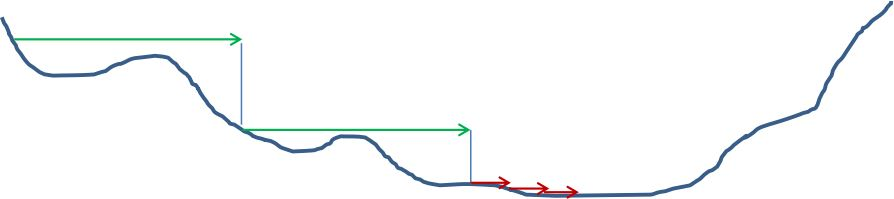
\includegraphics[width=0.75\textwidth]{gradientdescentlearningrate}
		\caption{.}
		\label{fig:gradientdescentlearningrate}
	\end{figure}

The challenge is, all the weights in all the inputs of all the neurons need to be adjusted. It is not manually possible to find the right combination of weights using brute force. Instead, the neural network algorithm uses a learning function called gradient descent.
	\begin{numberedlist}
		\item A random combination of bias B1 and input weights W1 (showing only one as more than one is not possible to visualize)
		\item Each combination of W1 and B1 is one particular linear model in a neuron. That model is associated with proportionate error e1 (red dashed line).
		\item Objective is to drive e1 towards 0. For which we need to find the optimal weight (Woptimal) and bias (Boptimal)
		\item The algorithm uses gradient descent algorithm to change bias and weight form starting values of B1 and W1 towards the Boptimal, Woptimal.
	\end{numberedlist}

 	\begin{figure}[h]
		\centering
		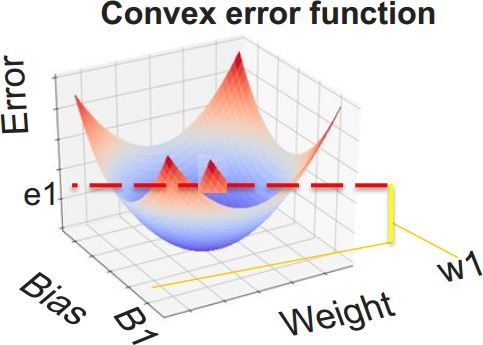
\includegraphics[height=1.5in]{gradientdescent3}
		\caption{.}
		\label{fig:gradientdescent3}
	\end{figure}

 	\begin{figure}[h]
		\centering
		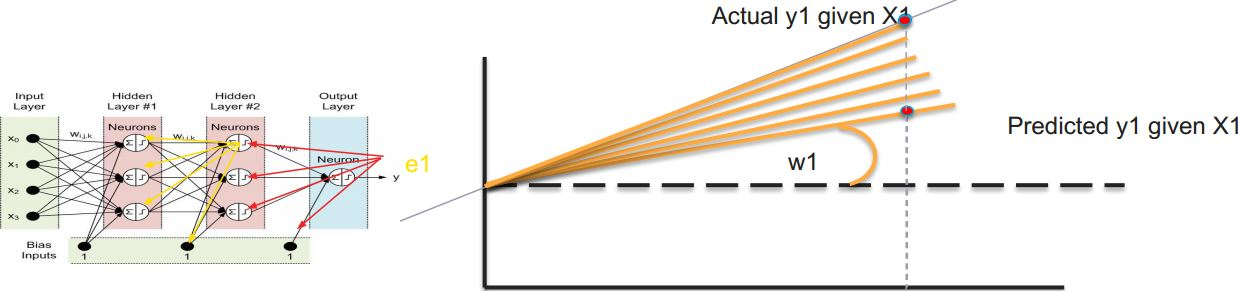
\includegraphics[width=0.75\textwidth]{gradientdescent4}
		\caption{.}
		\label{fig:gradientdescent4}
	\end{figure}


	\begin{bulletedlist}
		\item Let target value for a training example $X$ be $y$ i.e., the data frame used for training has value $X$, $y$.
		\item Let the model (represented by random m and c) predict the value for the training example $X$ to be $\hat{y}$.
		\item Error in prediction is $E = \hat{y} - y$. If we sum all the errors across all data points, some will be positive some negative and thus cancel out.
		\item To prevent the sum of errors becoming 0, we square the error i.e.\ E = $(y - \hat{y})^2$. Note: in squared expression, $y - \hat{y}$ or $\hat{y} - y$ mean the same.
		\item Sum of $(y - \hat{y})^2$ across all the X values is called SSE (Sum of Squared Errors).
		\item Using gradient descent (descend towards the global minima). Gradient descent uses partial derivatives i.e.\ how the SSE changes on slightly modifying the model parameters m and c one at a time (see \equationname~\ref{eq:gradientdescent1}).
		\item Gradient descent is a way to minimize an objective function / cost function such as Sum of Squared Errors (SSE) that is dependent on model parameters of weight / slope and bias.
		\item The parameters are updated in the direction opposite to the direction of the gradient (direction of maximum increase) of the objective function.
		\item In other words we change the values of weight and bias following the direction of the slope of the surface of the error function down the hill until we reach minima.
		\item This movement from starting weight and bias to optimal weight and bias may not happen in one shot.  It is likely to happen in multiple iterations. The values change in steps.
		\item The step size can be influenced using a parameter called Learning Rate. It decides the size of the steps i.e. the amount by which the parameters are updated. Too small  learning step will slow down the entire process while too large may lead to an infinite loop.
		\item The mathematical expression of gradient descent.
	\end{bulletedlist}

	\begin{align}
		d(E) / d(m) &= d(sum(\hat{y} - y)^2) / d(m) \\
		d(E) / d(c) &= d(sum(\hat{y} - y)^2) / d(c)
		\label{eq:gradientdescent1}
	\end{align}

	\begin{figure}[h]
		\centering
		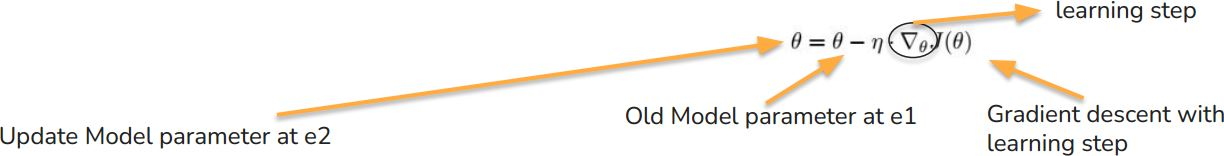
\includegraphics[width=0.75\textwidth]{gradientdescent5}
		\caption{.}
		\label{fig:gradientdescent5}
	\end{figure}


Transform our error function (which is a quadratic / convex function) into a contour graph. Gradient is
always found on the input model parameters only:

	\begin{bulletedlist}
		\item Every ring on the error function represents a combination of coefficients (m1 and m2 in the image) which result in same quantum of error i.e.\ SSE.
		\item Let us convert that to a 2d contour plot. In the contour plot, every ring represents one quantum of error.
		\item The innermost ring / bull's eye is the combination of the coefficients that gives the lease SSE.
	\end{bulletedlist}

	\begin{figure}[h]
		\centering
		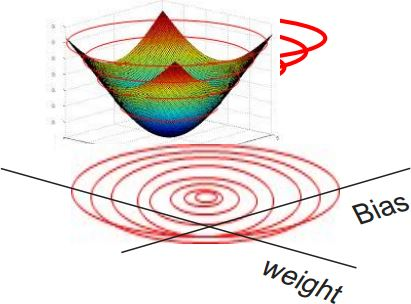
\includegraphics[height=2.0in]{gradientdescent6}
		\caption{.}
		\label{fig:gradientdescent6}
	\end{figure}

About the contour graph (\figurename~\ref{fig:gradientdescent7}):
	\begin{bulletedlist}
		\item Outermost circle is highest error while innermost is the least error circle.
		\item A circle represents combination of parameters which result in same error. Moving on a circle will not reduce error.
		\item Objective is to start from anywhere but reach the innermost circle.
	\end{bulletedlist}


	\begin{figure}[h]
		\centering
		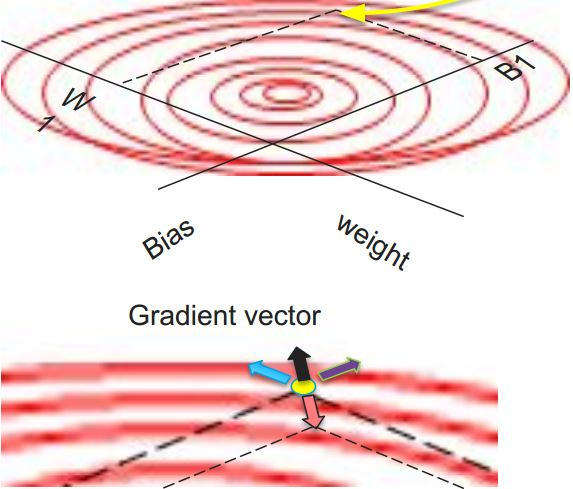
\includegraphics[height=2.0in]{gradientdescent7}
		\caption{.}
		\label{fig:gradientdescent7}
	\end{figure}


Gradient Descent Steps

	\begin{numberedlist}
		\item First evaluate dy(error)/d(weight) to find the direction of highest increase in error given a unit change in weight (Blue arrow). Partial derivative w.r.t.\ to weight
		\item Next find dy(error)/d(bias) to find the direction of highest increase in error given a unit change in bias (green arrow). Partial derivative w.r.t.\ to bias
		\item Partial derivatives give the gradient in the given axis and gradient is a vector
		\item Add the two vectors to get the direction of gradient (black arrow) i.e.\ direction of max increase in error
		\item We want to decrease error, so find negative of the gradient i.e.\ opposite to black arrow (orange arrow).  The arrow tip is new value of bias and weight.
		\item Recalculate the error at this combination an iterate to step 1 till movement in any direction only increases the error.
	\end{numberedlist}


	\section{Drawbacks of Artificial Neural Networks}

	\begin{bulletedlist}
		\item ANN models are not much interpretable so it does not give any clue on how it has come up with a solution. Thus it does not make ANN models reliable or trustworthy.
		\item There is no specific rule for determining the architecture of the network so we mostly use hit and trial method.
		\item In-order to work efficiently, ANN requires parallel computing power.
		\item ANN can only work with numerical data so problems or data need to be converted into numerical format before feeding it to ANN.
		\item Duration of the model to train on the data takes longer.
	\end{bulletedlist}

	\section{Why Deep Learning Over Traditional Machine Learning?}

Deep Learning is considered as a subset of machine learning since it achieves the same goal, allowing machines to learn from data in order to gain useful insights. However, a very common question that arises is - Why move to neural networks when we had the traditional machine learning algorithms? So let us have a look at the differences now.

	\begin{numberedlist}
		\item Feature Engineering
		\begin{bulletedlist}
			\item Machine Learning requires extensive feature engineering for the model to perform better. On the other hand, Deep Learning learns to extract the relevant features from the data set.
		\end{bulletedlist}
		\item Performance with Data
		\begin{bulletedlist}
			\item Deep Learning performs poorly with lesser data but outshines the traditional machine learning algorithms with huge amounts of data. Since we are generating huge amounts of data every day, deep learning algorithms definitely perform better.
		\end{bulletedlist}
		\item Computation Requirements
		\begin{bulletedlist}
			\item Traditional machine learning algorithms generally have a low computational requirement. However, since there are a not of matrix multiplications required in the implementation of neural network-based learning, these algorithms are computationally extensive.
		\end{bulletedlist}
	\end{numberedlist}

Now, with the huge amounts of data being generated and extensive computation abilities being present, organizations are stressing on deep learning research work and most AI-based applications are finding their foundations in Neural Networks.
